\documentclass{beamer}

\usepackage[brazilian]{babel}
\usepackage[utf8]{inputenc}
\usepackage{graphicx}
\usepackage[T1]{fontenc}

\usepackage{hyperref}
\hypersetup{
  linkcolor=black,
  colorlinks=true,
  urlcolor=cyan
}


\usetheme{Frankfurt}
\usecolortheme{seagull}
\setbeamertemplate{navigation symbols}{}

%================================================================================
%================================================================================

\begin{document}
\title{Introdução ao Git} 
\author{Felipe dos Santos Silveira} 
\date{\today} 

\frame{
  \titlepage
} 

%% \frame{
%%   \frametitle{Table of contents}

%%   \tableofcontents
%% } 


%================================================================================
%================================================================================

\section{Introdução} 

\subsection{Histórico}
\frame{
  \frametitle{Histórico} 

  Criado por Linus Torvalds para desenvolvimento do Kernel Linux

  \begin{itemize}
    \item Distribuído
    \item Apto ao desenvolvimento não linear
    \item Trabalha eficientemente (tempo e espaço) com projetos grandes
  \end{itemize}
}


\subsection{Conceitos}
\frame{
  \frametitle{Características} 
  
  \begin{itemize}
    \item Armazena snapshots de arquivos e não diferença entre versões
    \item Maioria das operações são locais
    \item Mantém integridade (via hashes SHA-1)
    \item Dados só são adicionados ao repositório
  \end{itemize}   

}

\frame{
  \frametitle{Estados de modificações}

  Existem 3 estados em que uma modificação pode estar

  \begin{block}{working tree}
    Mudanças, arquivos adicionados, arquivos removidos.
  \end{block}

  \begin{block}{Staging area}
    Snapshots de arquivos da working tree que serão commitados.
  \end{block}

  \begin{block}{Repositório}
    Aqui ficam armazenados os commits feitos. De maneira geral, eles não são mais editados.
  \end{block}

}


\frame {
  \frametitle{Estrutura de um commit}

  Um commit é composto por quatro partes: 
  \begin{itemize}
    \item Autor, informações do commiter, data
    \item Um snapshot dos arquivos do repositório
    \item Uma mensagem de commit
    \item Uma lista de commits do qual ele derivou
  \end{itemize} 

  À partir dessas informações é calculado o hash SHA-1, que é usado para identificar unicamente esse commit.
  

}


\frame{
  \frametitle{Exemplo de commits}

  \begin{center}
    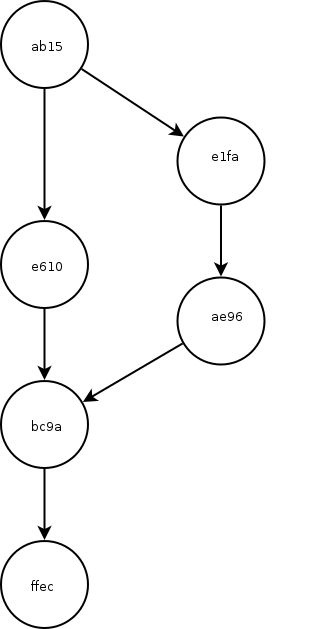
\includegraphics[width=\textwidth,height=0.8\textheight,keepaspectratio]{Imagens/ex-repo.png}
  \end{center}

}


%================================================================================
%================================================================================


\section{Configurações}
\subsection{Instalação}


\frame{
  \frametitle{Instalação}

  Veja como instalar na sua distribuição/sistema operacional no site oficial: \href{http://git-scm.com/downloads}{git-scm.com/downloads}
  
}


\frame{
  \frametitle{Configuração}

  Antes de começar a trabalhar precisamos nos identificar.

  Para isso usamos o comando \textbf{git config}

  \begin{block}{Definindo variáveis de usuário}
    \textbf{git config -{}-global user.name ``<Seu nome>''}\\
    \textbf{git config -{}-global user.email ``<Seu email>''}\\
    \textbf{git config -{}-global core.editor ``gedit''}\\
  \end{block}

}


\frame{
  \frametitle{Níveis de configuração}
  
  Existem 3 níveis de configuração:

  \begin{itemize}
    \item \textbf{local} para configurações somente para o repositório atual
    \item \textbf{global} para configurações somente para o usuário atual
    \item \textbf{system} para configurações para todos usuários do sistema
  \end{itemize}

}

%================================================================================
%================================================================================

\section{Primeiros passos}
\subsection{Comandos}

\frame {
  \frametitle{git init}

  Um repositório é criado executando o comando \textbf{git init}.\\
  
  Durante este mini-curso, utilizares um repositório de exemplo.
  \begin{alertblock}{Execute}
    \textbf{git clone https://github.com/berr/minicurso-git.git}
  \end{alertblock}  
}


\frame{
  \frametitle{git add}

  As mudanças são adicionadas na \textbf{staging area} utilizando o comando \textbf{git add <arquivo>}

  \begin{alertblock}{Lembre-se}
    Um snapshot do arquivo é guardado na \textbf{staging area}. Caso mais modificações sejam feitas, elas precisam ser adicionadas de novo.
  \end{alertblock}

  \begin{alertblock}{Dica}
    O comando \textbf{git add .} adiciona recursivamente todos os arquivos do diretório atual e seus sub-diretórios à staging area.
  \end{alertblock}

}

\frame{
  \frametitle{git status e git diff}

  Como está a nossa \textbf{working tree} e \textbf{staging area}?

  \begin{itemize}
    \item O comando \textbf{git status} nos mostra o estado atual do repositório, além de algumas outras dicas, que veremos em breve. 

    \item O comando \textbf{git diff} nos mostra as diferenças entre a \textbf{working tree} e o último commit. 
    \item Para ver mudanças apenas da \textbf{staging area} use \textbf{git diff -{}-cached}.
  \end{itemize}

}


\frame{
  \frametitle{git rm}

  Às vezes precisamos remover um arquivo do nosso repositório.
  Podemos atingir esse objetivo com o comando \textbf{git rm <arquivo>}

  \begin{alertblock}{Cuidado}
    O comando \textbf{git rm} também deleta o arquivo do sistema. \\
    Utilize a \textbf{git rm -{}-cached <arquivo>} para manter ele em disco.
  \end{alertblock}

  \begin{alertblock}{Lembre-se}
    As operações do git são aditivas. Logo, ainda é possível recuperar o arquivo deletado.
  \end{alertblock}

}

\frame{
  \frametitle{git commit}

  Com as mudanças adicionadas à \textbf{staging area} podemos fazer o nosso primeiro commit com \textbf{git commit}

  O editor que configuramos com \emph{core.editor} será chamado e poderemos ver os arquivos modificados e editar a mensagem de commit.

  \begin{block}{Boa prática}
    Uma boa mensagem de commit é composta de duas partes separadas por uma linha em branco: Uma mensagem de até 80 caracteres que descreve brevemente o commit. E, se necessário, uma melhor descrição após uma linha em branco.
  \end{block}

  \begin{block}{Commit message}
    A mensagem do commit também pode ser passada por parâmetro. \textbf{git commit -m <commit message>}
  \end{block}
  
}

\frame{
  \frametitle{Commit temporário}

  O comando \textbf{git stash} permime guardar as modificações locais rapidamente para, por exemplo, poder trocar de branch.

  \begin{block}{git stash}
    Guarda as modificações locais em uma pilha
  \end{block}

  \begin{block}{git stash pop}
    Remove a última modificação guardada com \textbf{git stash} e aplica na \textbf{working tree}
  \end{block}
  

}

\frame{
  \frametitle{git log}

  A qualquer momento podemos ver como está o repositório com o comando \textbf{git log}

  \begin{block}{Formatação}
    A saída do comando é totalmente configurável. Não esqueça de ver as opções com \textbf{git help log}.

    A minha formatação preferida: \textbf{git log -{}-pretty=format:``\%h \%ad | \%s\%d [\%an]'' -{}-graph -{}-date=short}
  \end{block}

}


%================================================================================
%================================================================================

\section{Conceitos}

\subsection{Navegação}


\frame{
  \frametitle{Referências}

  Como você deve ter percebido, todos os commits são referenciados por seus hashes. Porém, podemos usar um modo mais amigável de referenciá-los.
  Para isso, usamos \textbf{Referências}, que são ponteiros para commits. Existem 3 tipos de referências:

  \begin{itemize}
    \item \textbf{tag}: Um ponteiro para um commit específico. Ela não se move sob qualquer circunstância.
    \item \textbf{branch}: Um ponteiro para uma ``linha'' de commits. É atualizado quando há um novo commit no branch.
  \end{itemize}
}

\frame{
  \frametitle{HEAD}

  \textbf{HEAD} é a referência para onde estamos. Pode estar em dois estados:

  \begin{itemize}
    \item Apontando para um branch. Assim, os commits feitos à partir de HEAD atualizarão o ponteiro do branch.
    \item Apontando para uma tag ou commit. Esse estado é chamado de \textbf{detached HEAD} e os commits feitos só serão alcançáveis à partir de seus hashes.
  \end{itemize}

}


\frame{
  \frametitle{Um repositório com referências}

  \begin{center}
    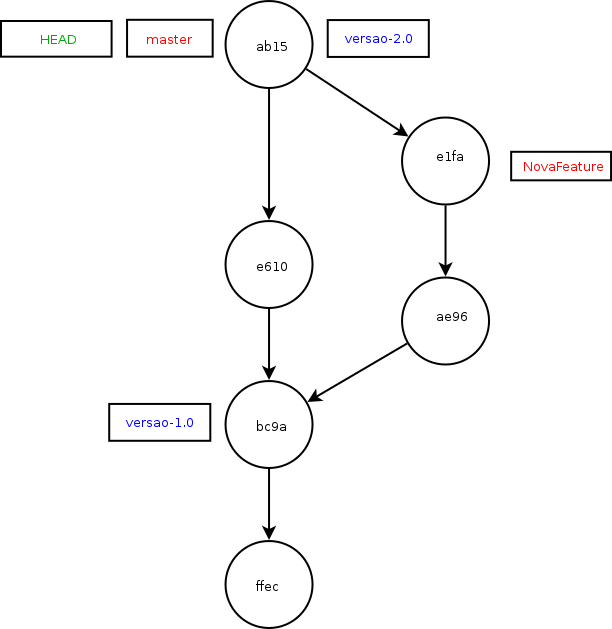
\includegraphics[width=\textwidth,height=0.8\textheight,keepaspectratio]{Imagens/ex-refs.png}
  \end{center}

}

\frame{
  \frametitle{git checkout}

  Move o ponteiro de HEAD para a o destino especificado (branch, tag, commit)

  \begin{block}{Obtendo um arquivo de outro commit}
    Para trazer para a \textbf{working tree} o arquivo X no commit Y, execute \textbf{git checkout Y -{}- X}.
  \end{block}

  \begin{block}{Dica}
    O comando \textbf{git reflog} mostra o histórico do ponteiro \textbf{HEAD}, e é útil para se recuperar em situações desastrosas.
  \end{block}  

}

\frame{
  \frametitle{git reset}

  Move o pointeiro do branch atual.

  \begin{block}{Cuidado}
    O comando reset move o ponteiro do branch, e não a referência de HEAD, como o checkout. Ou seja, os commits do branch antigo não serão mais alcançados.
  \end{block} 

}

\frame{
  \frametitle{git reset -{}-hard versao-1.0}

  \begin{center}
    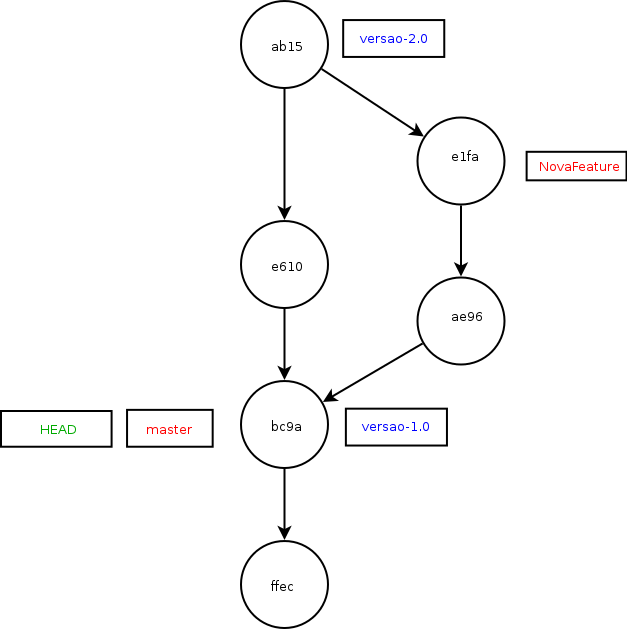
\includegraphics[width=\textwidth,height=0.8\textheight,keepaspectratio]{Imagens/ex-reset.png}
  \end{center}  

}

\frame{
  \frametitle{Criando referências}

  \begin{block}{Criando uma tag à partir do commit apontado por \textbf{HEAD}}
    \textbf{git tag <nome-da-tag>}
  \end{block}

  \begin{block}{Criando um branch à partir do commit apontado por \textbf{HEAD}}
    \textbf{git checkout -b <nome-do-branch>}
  \end{block}

}


\subsection{Gerenciando branches}

\frame{
  \frametitle{git merge}
  
  Um ``merge`` é um ponto onde duas linhas separadas se encontram. Ou seja, é a junção de dois branches para criar um commit que terá dois pais.

  \begin{block}{Exemplo}
    \textbf{git merge NovaFeature}
  \end{block}


  \begin{block}{fast forward}
    Quando o alvo do comando for um sucessor direto do branch commit atual, o merge é chamado de \textbf{fast forward} e somente as referências são atualizadas.
  \end{block}

}

\frame{
  \frametitle{Conflitos}

  Caso haja um conflito que o git não consiga resolver, o arquivo com conflito será alterado para que possamos tomar providências.
  
  \begin{block}{Lembre-se}
    O comando \textbf{git status} nos dá informações sobre conflitos que ocorreram.
  \end{block}  

}

\frame{
  \frametitle{git rebase}

  O comando rebase nos permite aplicar nossas mudanças partindo de outro commit base.

  \begin{block}{Exemplo}
    \textbf{git rebase <branch>}
  \end{block}

}


\frame{
  \frametitle{Estado inicial}

  \begin{center}
    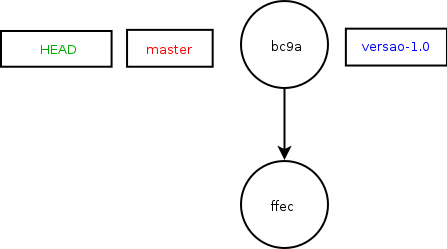
\includegraphics[width=\textwidth,height=0.4\textheight,keepaspectratio]{Imagens/ex-rebase1.png}
  \end{center}
}


\frame{
  \frametitle{Após algum tempo}

  \begin{center}
    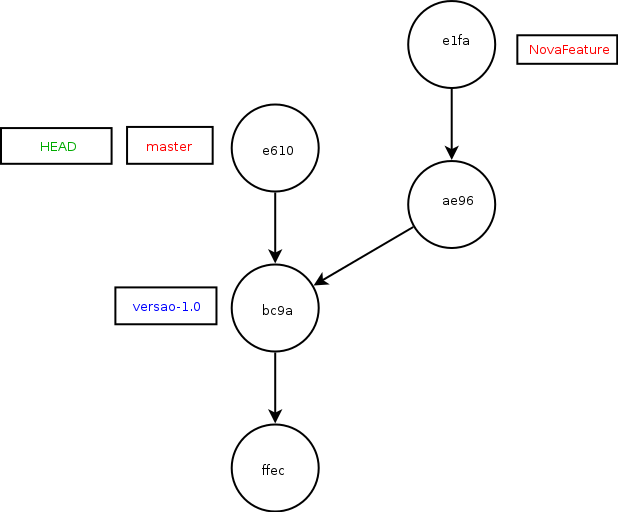
\includegraphics[width=\textwidth,height=0.8\textheight,keepaspectratio]{Imagens/ex-rebase2.png}
  \end{center}
}


\frame{
  \frametitle{Após o rebase}

  \begin{center}
    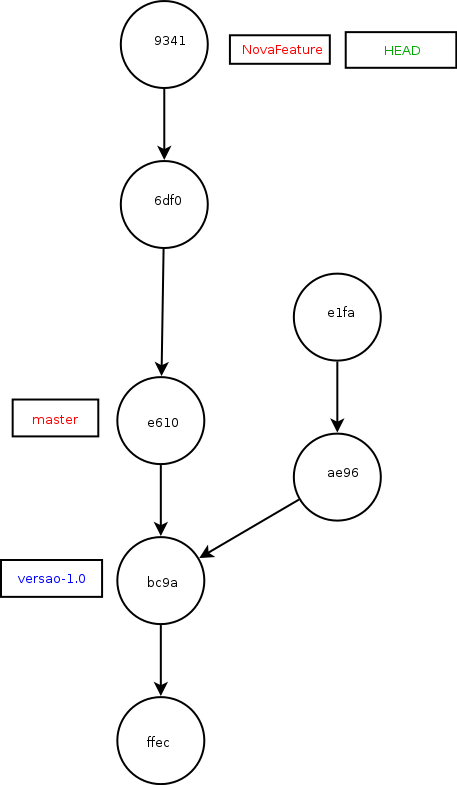
\includegraphics[width=\textwidth,height=0.8\textheight,keepaspectratio]{Imagens/ex-rebase3.png}
  \end{center}
}

\frame{
  \frametitle{Mais rebase}

  Você ainda pode usar a opção \textbf{-i} para editar os commits que serão adicionados.

  \begin{itemize}
    \item \textbf{reword}: mudar a mensagem do commit
    \item \textbf{edit}: parar para editar o commit 
    \item \textbf{squash}: junta com o commit anterior (mantém ambas mensagens)
    \item \textbf{fixup}: junta com o commit anterior (usa só a mensagem do anterior)    
  \end{itemize}

  Se um linha for apagada, o commit não será usado. \\
  Os commits são aplicados de cima para baixo, e podem ser reordenados à vontade.

}

\section{Servidores Remotos}

\subsection{}

\frame{
  \frametitle{git clone}

  O comando \textbf{git clone} faz uma cópia de um repositório externo para a sua máquina.

  \begin{block}{Clonando o repositório do linux}
    \textbf{git clone git://github.com/torvalds/linux.git}
  \end{block}
  

}

\frame{
  \frametitle{Sincronização}

  Como as operações são sempre locais, precisamos de algum modo pra sincronizar os repositórios.

  \begin{itemize}
    \item \textbf{git fetch}: apenas baixa as informações sobre os servidores remotos
    \item \textbf{git pull}: a mesma coisa que \textbf{fetch}, mas faz merge do branch atual com o seu respectivo remoto.
    \item \textbf{git push}: atualiza os servidores remotos com as mudanças locais
  \end{itemize}

}

\frame{
  \frametitle{Referências remotas}

  As referências de servidores remotos têm como prefixo o nome do servidor remoto.\\
  O nome do primeiro \textbf{remote} geralmente é ``origin''.

  
  \begin{center}
    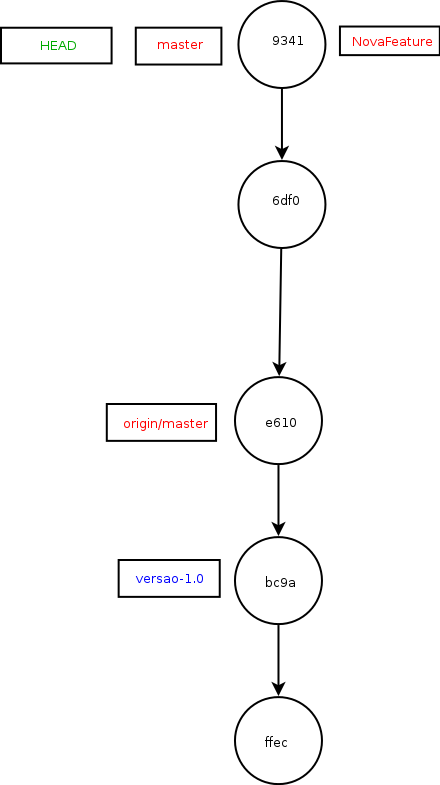
\includegraphics[width=\textwidth,height=0.7\textheight,keepaspectratio]{Imagens/ex-remote.png}
  \end{center}


}


\frame{
  \frametitle{git pull}

  Assumindo que o branch local seja ``master''

  \begin{block}{Equivalente a}
    \textbf{git fetch}\\
    \textbf{get merge origin/master}
  \end{block}

  Gera muitos commits de merge em um repositório ativo.
  
}

\frame{
  \frametitle{git push}
  
  Somente commits que sejam \textbf{fast forward} serão atualizados no servidor.

  \begin{block}{Criando um branch remoto}
    \textbf{git push -u <remote> <branch-local>} \\
    A opção \textbf{-u} configura o seu repositório para associar o branch remoto ao local.
  \end{block}

  \begin{block}{Deletando um branch remoto}
    \textbf{git push <remote> :<branch-remoto>}
  \end{block}

  \begin{block}{Enviando tags}
    \textbf{git push <remote> <tag-local>}.\\
    Note: A opção \textbf{-{}-tags} transferirá \textbf{todas} as tags locais para o servidor.
  \end{block}
}


\section{Outros}

\subsection{Hospedagem}

\frame{
  \frametitle{}

  \begin{block}{GitHub}
    \href{https://github.com/}{https://github.com/}\\

    Conta com repositórios privados gratuita em: \href{https://github.com/edu}{https://github.com/edu}
  \end{block}

  \begin{block}{BitBucket}
    \href{https://bitbucket.org}{https://bitbucket.org}
  \end{block}
}

\subsection{Ferramentas}

\frame{

  \frametitle{}
  
  \begin{itemize}
    \item \href{http://www.eclipse.org/egit/}{EGit} --  Plugin para eclipse
    \item \textbf{git-gui} -- Geralmente distribuído com o git
    \item \href{http://code.google.com/p/gitextensions}{GitExtensions} -- Front-end gráfico para windows
    \item Mais informações na \href{https://git.wiki.kernel.org/index.php/Interfaces,_frontends,_and_tools}{wiki oficial}
  \end{itemize}

}


\end{document}

